\documentclass[12pt]{article}%{bmcart}
\usepackage[doublespacing]{setspace}
\usepackage[a4paper]{geometry}
\usepackage{textcomp}
\usepackage{adjustbox,lipsum}
\geometry{verbose,tmargin=2cm,bmargin=2cm,lmargin=2cm, rmargin=2cm}
\usepackage{amsthm,amsmath}
\RequirePackage{natbib}
\bibliographystyle{apalike}
\usepackage{longtable}
\usepackage{cite}
\usepackage{booktabs}
\RequirePackage{hyperref}
\usepackage[utf8]{inputenc}
\usepackage[document]{ragged2e}
\usepackage{lineno}


\usepackage{graphicx}
\usepackage{verbatim}
\usepackage{float}
%\usepackage{tabular}
\usepackage[section]{placeins}
\usepackage{placeins}
\usepackage{color, colortbl}
\usepackage{caption}
\usepackage{subcaption}
\usepackage{parskip}

\renewcommand\thefigure{S\arabic{figure}} 

\renewcommand\thetable{S\arabic{table}} 

\title{Supplementary information for ``Quantifying influences on intragenomic mutation rate"}

\author{Helmut Simon \& Gavin A Huttley}

\begin{document}
\maketitle

\newpage

\begin{table}[htp!]
\centering
\begin{tabular}{ c c c c c c c c c }
\hline
\bf{Chr} & \bf{SNV density} & \bf{p} & \bf{q} & \bf{Slope} & \bf{Intercept} & \bf{$\hat{\sigma }^2_{rec}$} & \bf{Slope (M)} & \bf{Percent} \\
\hline
\hline
  1 &      0.0252 &  8 & 2 & 0.0085 &    0.0251 &                3.08e-07 &  3.74e-09 & 0.431\% \\
  2 &      0.0260 & 10 & 3 & 0.0072 &    0.0259 &                2.07e-07 &  3.46e-09 & 0.265\% \\
  3 &      0.0262 &  9 & 4 & 0.0072 &    0.0261 &                1.87e-07 &  3.45e-09 & 0.326\% \\
  4 &      0.0267 & 10 & 4 & 0.0061 &    0.0267 &                1.51e-07 &  2.88e-09 & 0.239\% \\
  5 &      0.0261 &  8 & 4 & 0.0075 &    0.0260 &                1.76e-07 &  3.48e-09 & 0.347\% \\
  6 &      0.0263 &  3 & 2 & 0.0062 &    0.0263 &                8.05e-08 &  2.90e-09 & 0.248\% \\
  7 &      0.0262 &  9 & 2 & 0.0088 &    0.0261 &                3.07e-07 &  4.10e-09 & 0.452\% \\
  8 &      0.0274 &  6 & 4 & 0.0085 &    0.0272 &                2.78e-07 &  4.12e-09 & 0.594\% \\
  9 &      0.0254 &  4 & 4 & 0.0085 &    0.0253 &                6.25e-07 &  3.58e-09 & 0.478\% \\
 10 &      0.0263 &  5 & 4 & 0.0077 &    0.0262 &                3.07e-07 &  3.62e-09 & 0.245\% \\
 11 &      0.0269 &  3 & 3 & 0.0087 &    0.0268 &                1.57e-07 &  3.95e-09 & 0.379\% \\
 12 &      0.0252 &  5 & 4 & 0.0074 &    0.0251 &                2.18e-07 &  3.55e-09 & 0.281\% \\
 13 &      0.0261 &  7 & 4 & 0.0080 &    0.0260 &                2.22e-07 &  3.12e-09 & 0.377\% \\
 14 &      0.0264 &  8 & 3 & 0.0092 &    0.0263 &                2.33e-07 &  3.53e-09 & 0.412\% \\
 15 &      0.0261 &  2 & 2 & 0.0079 &    0.0260 &                4.88e-07 &  3.18e-09 & 0.432\% \\
 16 &      0.0286 & 10 & 4 & 0.0083 &    0.0285 &                1.22e-06 &  3.65e-09 & 0.519\% \\
 17 &      0.0256 & 10 & 1 & 0.0090 &    0.0255 &                6.02e-07 &  4.13e-09 & 0.509\% \\
 18 &      0.0265 &  4 & 2 & 0.0067 &    0.0264 &                2.31e-07 &  3.01e-09 & 0.383\% \\
 19 &      0.0275 &  8 & 4 & 0.0071 &    0.0274 &                1.91e-07 &  3.13e-09 & 0.413\% \\
 20 &      0.0265 &  9 & 3 & 0.0076 &    0.0264 &                2.84e-07 &  3.37e-09 & 0.468\% \\
 21 &      0.0275 &  2 & 2 & 0.0067 &    0.0274 &                1.73e-07 &  2.17e-09 & 0.428\% \\
 22 &      0.0272 &  7 & 3 & 0.0069 &    0.0271 &                5.28e-07 &  2.27e-09 & 0.437\% \\
\hline
\end{tabular}
\caption{Results of analysis of variance due to recombination by chromosome. `p' and `q' define the ARMA(p,q) distribution used; `Slope' and `Intercept' are the estimated parameters of the linear model expressed in terms of change in SNV density per centimorgan and SNV density respectively; `$\hat{\sigma }^2_{rec}$' is the estimated variance in SNV density due to recombination; `Slope (M)' is the estimated slope parameter expressed as change in mutation rate per centimorgan; and `Percent' is the estimated percentage of SNVs due to recombination. }
\label{tab:supp-recomb}
\end{table}


\newpage

\begin{table}[htp!]
\centering
\begin{adjustbox}{max width=\textwidth}
\begin{tabular}{ l c c c c c c c c c c c c }
\hline
\bf{} & \bf{C\textrightarrow T} & \bf{G\textrightarrow A} & \bf{T\textrightarrow C} & \bf{A\textrightarrow G} & \bf{C\textrightarrow G} & \bf{G\textrightarrow C} & \bf{T\textrightarrow G} & \bf{A\textrightarrow C} & \bf{T\textrightarrow A} & \bf{A\textrightarrow T} & \bf{C\textrightarrow A} & \bf{G\textrightarrow T} \\
\hline
\hline
 1 &               0.00 &               0.00 &               0.00 &               0.00 &               0.00 &               0.00 &               0.01 &               0.02 &               0.95 &               0.37 &               0.91 &               0.93 \\
 2 &               0.00 &               0.00 &               0.00 &               0.00 &               0.00 &               0.01 &               0.04 &               0.00 &               0.15 &               0.16 &               0.84 &               0.99 \\
 3 &               0.00 &               0.00 &               0.00 &               0.00 &               0.00 &               0.26 &               0.08 &               0.00 &               0.82 &               0.99 &               0.99 &               0.59 \\
 4 &               0.00 &               0.00 &               0.00 &               0.00 &               0.01 &               0.01 &               0.11 &               0.00 &               0.94 &               0.66 &               0.99 &               0.62 \\
 5 &               0.00 &               0.00 &               0.00 &               0.00 &               0.00 &               0.02 &               0.00 &               0.00 &               0.28 &               0.74 &               0.98 &               0.95 \\
 6 &               0.00 &               0.00 &               0.00 &               0.00 &               0.07 &               0.11 &               0.06 &               0.06 &               0.99 &               0.58 &               0.99 &               1.00 \\
 7 &               0.00 &               0.00 &               0.00 &               0.00 &               0.15 &               0.00 &               0.04 &               0.00 &               0.82 &               0.65 &               0.62 &               0.76 \\
 8 &               0.00 &               0.00 &               0.00 &               0.00 &               0.05 &               0.04 &               0.02 &               0.00 &               0.47 &               0.06 &               0.91 &               0.96 \\
 9 &               0.00 &               0.00 &               0.00 &               0.00 &               0.01 &               0.01 &               0.10 &               0.02 &               0.40 &               0.25 &               0.48 &               0.99 \\
10 &               0.00 &               0.00 &               0.00 &               0.00 &               0.25 &               0.01 &               0.00 &               0.07 &               0.30 &               0.59 &               0.55 &               0.94 \\
11 &               0.00 &               0.00 &               0.00 &               0.00 &               0.69 &               0.00 &               0.80 &               0.38 &               0.24 &               0.31 &               0.88 &               0.94 \\
12 &               0.00 &               0.00 &               0.00 &               0.00 &               0.03 &               0.01 &               0.15 &               0.37 &               0.71 &               0.48 &               0.22 &               0.56 \\
13 &               0.00 &               0.00 &               0.00 &               0.00 &               0.01 &               0.03 &               0.00 &               0.01 &               0.03 &               0.26 &               0.57 &               0.90 \\
14 &               0.00 &               0.00 &               0.00 &               0.00 &               0.01 &               0.21 &               0.00 &               0.00 &               0.05 &               0.96 &               0.81 &               0.73 \\
15 &               0.00 &               0.00 &               0.00 &               0.00 &               0.42 &               0.45 &               0.16 &               0.16 &               0.44 &               0.10 &               0.09 &               0.13 \\
16 &               0.00 &               0.00 &               0.00 &               0.00 &               0.02 &               0.38 &               0.03 &               0.00 &               0.99 &               0.50 &               0.95 &               0.62 \\
17 &               0.00 &               0.00 &               0.00 &               0.00 &               0.01 &               0.00 &               0.37 &               0.00 &               0.19 &               0.19 &               0.19 &               0.87 \\
18 &               0.00 &               0.00 &               0.00 &               0.00 &               0.01 &               0.21 &               0.04 &               0.05 &               0.38 &               0.24 &               0.77 &               0.53 \\
19 &               0.00 &               0.00 &               0.02 &               0.00 &               0.04 &               0.38 &               0.82 &               0.07 &               0.27 &               0.00 &               0.85 &               0.96 \\
20 &               0.00 &               0.00 &               0.00 &               0.00 &               0.00 &               0.07 &               0.00 &               0.01 &               0.61 &               0.86 &               0.88 &               0.53 \\
21 &               0.00 &               0.02 &               0.00 &               0.00 &               0.20 &               0.00 &               0.18 &               0.11 &               0.88 &               0.00 &               0.01 &               0.79 \\
22 &               0.01 &               0.00 &               0.00 &               0.00 &               0.03 &               0.08 &               0.05 &               0.09 &               0.03 &               0.33 &               0.36 &               0.23 \\
\hline
\end{tabular}
\end{adjustbox}
\caption{Posterior probability that recombination does not have a positive effect on mutation               by point mutation direction and chromosome. }
\label{supp_recombination_chromosomes}
\end{table}



\newpage

\begin{table}[htp!]
\centering
\begin{tabular}{ c c c c c }
\hline
\bf{Mutation} & \bf{Density} & \bf{$\hat{\sigma }^2_3$} & \bf{$\hat{\sigma }^2_5$} & \bf{$\hat{\sigma }^2_7$} \\
\hline
\hline
C\textrightarrow T &  0.0207 &            6.13e-04 &            6.66e-04 &            7.82e-04 \\
C\textrightarrow A &  0.0045 &            6.14e-06 &            9.58e-06 &            1.37e-05 \\
C\textrightarrow G &  0.0054 &            1.07e-05 &            1.49e-05 &            2.07e-05 \\
T\textrightarrow C &  0.0093 &            8.24e-06 &            2.05e-05 &            2.89e-05 \\
T\textrightarrow A &  0.0024 &            4.99e-07 &            1.54e-06 &            3.14e-06 \\
T\textrightarrow G &  0.0029 &            6.16e-07 &            1.16e-06 &            2.24e-06 \\
A\textrightarrow C &  0.0029 &            3.64e-07 &            7.66e-07 &            1.49e-06 \\
A\textrightarrow T &  0.0028 &            7.13e-07 &            1.72e-06 &            3.38e-06 \\
A\textrightarrow G &  0.0135 &            2.03e-05 &            5.99e-05 &            7.36e-05 \\
G\textrightarrow C &  0.0044 &            6.94e-06 &            1.02e-05 &            1.42e-05 \\
G\textrightarrow T &  0.0051 &            8.26e-06 &            1.26e-05 &            1.82e-05 \\
G\textrightarrow A &  0.0203 &            5.08e-04 &            5.52e-04 &            6.51e-04 \\
\hline
\end{tabular}
\caption{Variance in probability of SNVs due to context. $\hat{\sigma }^2_k$ denote the estimated variances for context size $k$. The size of context includes the central allele. Results are conditioned on mutation direction (ancestral and derived state). The column `Density' shows the density for each SNV direction (conditioned on the ancestral allele) for reference. See Methods and materials for data sources. }
\label{tab:supp_context}
\end{table}

\newpage

\begin{figure}[h!]
\begin{subfigure} {1.0\textwidth}
\center
\includegraphics[width=0.8\textwidth]{figs/correlation_plot_supp_b.eps}
\caption{}
\label{fig:autocorrelation-a}
\end{subfigure}
\begin{subfigure} {1.0\textwidth}
\center
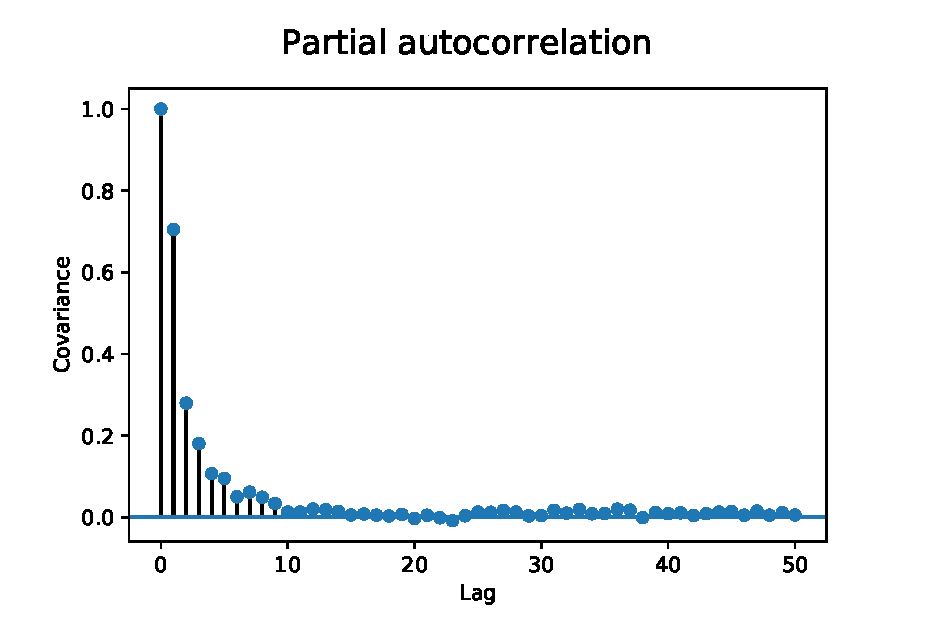
\includegraphics[width=0.8\textwidth]{figs/correlation_plot_supp_c.eps}
\caption{}
\label{fig:autocorrelation-b}
\end{subfigure}
\caption{Visualisation of auto-correlation of residuals from ordinary least squares linear regression of SNV densities against average recombination rates for chromosome 1. Correlation between residuals in bins separated by lags in the range 0 to 50 from (a) auto-correlation. (b) partial auto-correlation. The analysis removed the effect of correlations at shorter lags and indicates the number of lags required in an auto-regressive model (10 in this instance). The blue shading shows a 95\% significance interval.}
\label{fig:autocorrelation}
\end{figure}

\newpage

\begin{figure}[h!]
\center
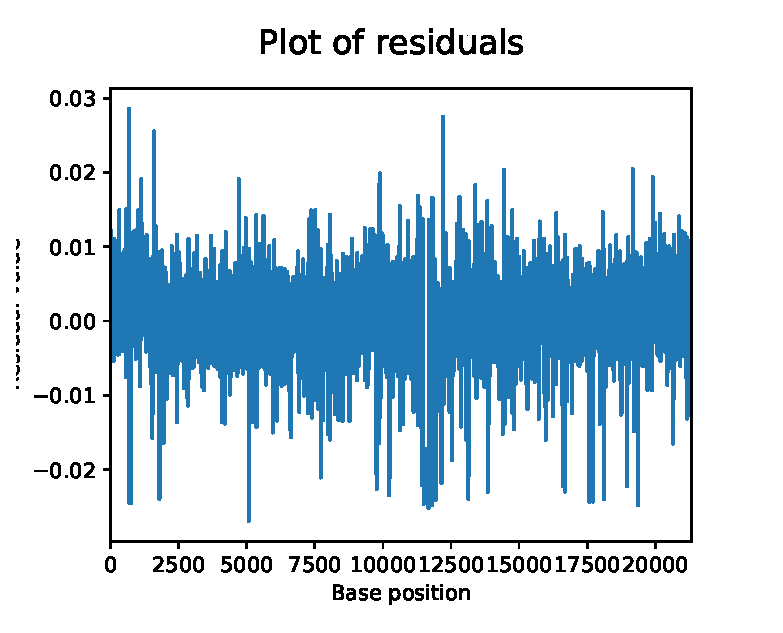
\includegraphics[width=0.8\textwidth]{figs/correlation_plot_supp_a.eps}
\caption{Visualisation of residuals of ordinary least squares linear regression of SNV densities against average recombination rates for chromosome 1 for 10-kb bins spanning the length of the chromosome. The residuals appear to have a constant mean of zero and a constant variance as required by stationarity. Stationarity is formally demonstrated by the Dickey-Fuller test.}
{\label{fig:residuals}}
\end{figure}

\newpage

\begin{table}[htp!]
\centering
\begin{tabular}{ c c c c c c c c }
\hline
\bf{Chr} & \bf{SNV density} & \bf{Slope} & \bf{Intercept} & \bf{$\hat{\sigma }^2_{rec}$} & \bf{Mutations} \\
\hline
\hline
  1 &      0.0252 & 0.0003 &    0.0249 &                  0.0225 &    0.0108 \\
  2 &      0.0260 & 0.0003 &    0.0258 &                  0.0169 &    0.0105 \\
  3 &      0.0262 & 0.0002 &    0.0260 &                  0.0193 &    0.0083 \\
  4 &      0.0267 & 0.0002 &    0.0266 &                  0.0145 &    0.0080 \\
  5 &      0.0261 & 0.0002 &    0.0259 &                  0.0123 &    0.0076 \\
  6 &      0.0263 & 0.0001 &    0.0262 &                  0.0052 &    0.0051 \\
  7 &      0.0262 & 0.0003 &    0.0259 &                  0.0187 &    0.0113 \\
  8 &      0.0274 & 0.0002 &    0.0272 &                  0.0113 &    0.0093 \\
  9 &      0.0254 & 0.0005 &    0.0249 &                  0.0262 &    0.0182 \\
 10 &      0.0263 & 0.0003 &    0.0260 &                  0.0188 &    0.0116 \\
 11 &      0.0269 & 0.0002 &    0.0267 &                  0.0096 &    0.0068 \\
 12 &      0.0252 & 0.0003 &    0.0250 &                  0.0136 &    0.0106 \\
 13 &      0.0261 & 0.0002 &    0.0259 &                  0.0245 &    0.0061 \\
 14 &      0.0264 & 0.0002 &    0.0262 &                  0.0237 &    0.0062 \\
 15 &      0.0261 & 0.0003 &    0.0257 &                  0.0315 &    0.0126 \\
 16 &      0.0286 & 0.0006 &    0.0278 &                  0.0466 &    0.0264 \\
 17 &      0.0256 & 0.0003 &    0.0252 &                  0.0454 &    0.0153 \\
 18 &      0.0265 & 0.0002 &    0.0263 &                  0.0260 &    0.0069 \\
 19 &      0.0275 & 0.0002 &    0.0272 &                  0.0093 &    0.0078 \\
 20 &      0.0265 & 0.0002 &    0.0262 &                  0.0262 &    0.0078 \\
 21 &      0.0275 & 0.0001 &    0.0274 &                  0.0172 &    0.0037 \\
 22 &      0.0272 & 0.0003 &    0.0267 &                  0.0347 &    0.0100 \\
\hline
\end{tabular}
\caption{Results of analysis of variance due to recombination by chromosome using ordinary last squares linear regression (OLSLR). `Slope' and `Intercept' are the estimated parameters of the linear model expressed in terms of change in SNV density per centimorgan and SNV density respectively; `$\hat{\sigma }^2_{rec}$' is the estimated variance in SNV density due to recombination; and `Mutations' is the estimated average number of mutations resulting from a recombination event. }
\label{tab:supp-OLSLR}
\end{table}

\newpage

\begin{table}[htp!]
\centering
\begin{tabular}{ c c c }
\hline
\bf{Chromosome} & \bf{Intronic variants} & \bf{All variants} \\
\hline
\hline
         1 &           2432041 &      5373514 \\
         2 &           2704243 &      5908524 \\
         3 &           2152067 &      4832711 \\
         4 &           1747006 &      4738393 \\
         5 &           1839945 &      4351659 \\
         6 &           1605617 &      4124061 \\
         7 &           1782609 &      3785873 \\
         8 &           1626541 &      3627183 \\
         9 &           1198502 &      2766514 \\
        10 &           1426815 &      3192424 \\
        11 &           1472265 &      3248165 \\
        12 &           1462768 &      3025811 \\
        13 &            823817 &      2214718 \\
        14 &            998643 &      1978949 \\
        15 &           1045461 &      1843388 \\
        16 &           1038676 &      1949903 \\
        17 &            961326 &      1725628 \\
        18 &            765211 &      1713065 \\
        19 &            668436 &      1234925 \\
        20 &            636129 &      1303247 \\
        21 &            358952 &       633564 \\
        22 &             19934 &       649010 \\
\hline
\end{tabular}
\caption{Counts of filtered variants by chromosome. Intronic variants were used for context analysis and all             variants were used for recombination analysis }
\label{tab:supp-counts}
\end{table}




\end{document}